\documentclass[12pt]{book}
\usepackage[a4paper,left=2cm,right=1cm,top=3cm,bottom=4cm,bindingoffset=5mm]{geometry}
\usepackage{fancyhdr}
%\usepackage{lscape} %für Querfromat
\usepackage{cancel} %um was in durchzustreichen
\usepackage{paralist} %um in enumerate einfach andere Sachen anzugeben
\usepackage{amsmath}
\usepackage{amssymb}
\usepackage{amsthm}
\usepackage{subcaption}
\usepackage{todonotes}
\usepackage[ngerman]{babel}
\usepackage[utf8]{inputenc}
%\usepackage{MnSymbol}
\usepackage{mathabx} % damit man Doppelklammern haben kann
\setlength{\parindent}{0em}  %verhindert Einrücken nach Absatz
\usepackage{xargs} %
\usepackage{tikz} %zum zeichnen
\usepackage{expdlist} % um den Zeilenabstand in description kleiner zu machen


\newcommand\tab[1][1cm]{\hspace*{#1}}

%\setmathfont[range={\lsem,\rsem}]{XITS Math}

% Meine Schrift, die mathe kann
\usepackage[math]{iwona}
\usepackage[T1]{fontenc}


\pagestyle{fancy}
\fancyhf{}
\lhead{Graph Drawing - Layer Assignment}
\rhead{ Thomas Dost, Jonas Lange, Francesca Rybicki}

\begin{document}
    
    \section*{Subject}
    
    %We aim to visualize the \textit{Layer Assignment} phase of the \textit{Layered} layout algorithm step by step.
    Unser Ziel ist es, die  \textit{Layer Assignment} Phase des \textit{Layered} Layout Algorithmus zu visualisieren. 
    Hierbei gibt die Graphische Schnittstelle dem Benutzer die Möglichkeit, den Algorithmus Schritt für Schritt betrachtet. 
    So soll der Benutzer durch Ausprobieren ein intuitives Verständnis für den Algorithmus entwickeln. Wichtig ist uns
    dabei, die verständliche Visualisierung des Algorithmus, so wie eine intuitiv zu bedienende GUI. Weniger wichtig ist
    uns eine gute Performance bei sehr großen Graphen, da für das Verständnis der \textit{Layer Assignment} Phase kleinere Graphen besser geeignet sind.
    
    
    
    \section*{Technische Umsetzung}
    
    Die technische Umsetzung ist in drei Schritte unterteilt:
    
    \begin{enumerate}
        \item first we parse\todo[inline]{THOMAS!! }
        \item Als nächstes wenden wir den \textit{Layer Assignment} Algorithmus auf den Elkgraphen an. Hierbei erstellen wir nach
        jedem Schritt einen SimpleGraph (vereinfachte Graphenstruktur, die nur die notwendigen Informeationen für die
        Visualisierung enthällt) aus dem Elkgraphen. Nachdem der \textit{Layer Assignment} Algorithmus fertig ist, geben wir 
        eine Liste dieser SimpleGraphs an die Visualisierung weiter.
        \item In der Visualisierung wird in jedem Schritt ein neuer SimpleGraph aus der Ausgabe des Algorithmus aus Schritt 2 geladen. Die Unterschiede, die zwischen zwei SimpleGraphs bestehen, werden dabei hervorgehoben. So ist es dem Benutzer möglich die Auswirkungen des Algorithmus in jedem Schritt nachzuvollziehen.
    \end{enumerate}
    
    Wie in folgendem Komponentendiagramm dargestellt, existieren Schnittstellen zwischen den einzelnen Berechnungsschritten, die die Datenweitergabe erlauben und an denen Überprüfungen vorgenommen werden, die sicher stellen, dass die weitere Berechnung möglich ist.
    
    
    \begin{figure}[ht!]
        \centering
        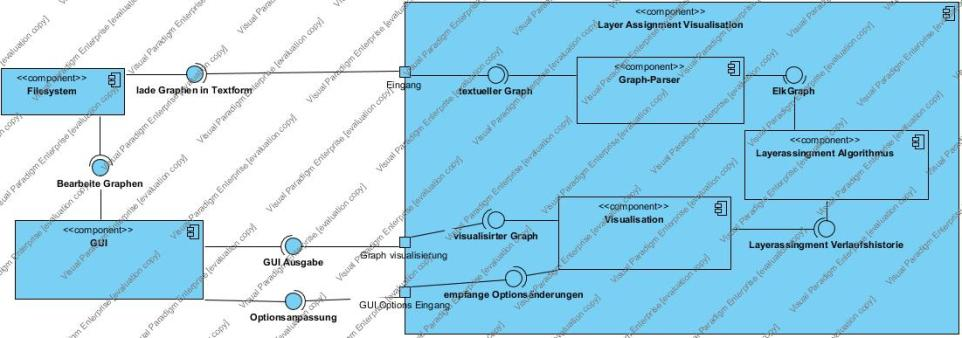
\includegraphics[width=\textwidth]{images/Component_Diagram1.jpg}
    \end{figure}
    
    
    
    



\subsection*{Parsing}
Die Parsing-Klasse ist dafür zuständig das eigens erstelle Textformate einzulesen
und in einen ElkGraph umzuwandeln, zusätlich wird der eingelesene Graph auf Kreisfreiheit überprüft
da der Layer-Assignment-Algorithmus nur für kreisfreie Graphen definiert ist.

\subsubsection*{Syntax}
Eine Node hinzufügen:
\newline
\tab[0.5cm]  node \_$<$node name$>$
\newline
\newline
Eine Edge hinzufügen:\newline
\tab[0.5cm]  edge\_$<$start node$>$ \_$<$end node$>$
\newline
Wobei \_ für beliebig viele Whitespaces steht,
weiter muss jeder Knoten der von einer edge benutzt wird vorher mit dem \textit{node} Keyword eingeführt werden

\subsubsection*{Methoden}
Parser.parse(<filepath>)\newline
Return: null falls ein fehler auftrat, sonst ein ElkGraph

\subsubsection*{Benutzung des Parsers}
try 
\{\newline
ElkNode testGraph = Parser.parse("testGraphs/testfile.txt");
\newline
\}
\newline
catch (Exception e)
\newline
\{
\newline
  e.printStackTrace(); 
\newline
\}


\subsubsection*{Beispiel}
node n1 \newline
node n2 \newline
node n3 \newline
\newline
\newline
edge n1 n3\newline 
edge n2 n3 \newline










    
    \documentclass[a4paper,10pt]{scrartcl}

\begin{document}
Die Klasse LayerAssignment enthällt eine Reihe hilfreicher Funktionen, die Wichtigste ist allerdings die Methode assignLayers. assignLayers nimmt einen ElkGraphen, führt das Layerassignment an ihm durch und gibt eine Bearbeitungshistorie in Form einer ArrayList vom typen MyGraph zurück. Wobei MyGraph eine von uns entwickelte vereinfachte Graphenstruktur ist. Jeder MyGraph in der Liste stellt also einen "snapshot" aus dem Layerassingments des Graphen dar.
Durch Seiteneffekte beinflusst die Methode auch den eingegebenen ElkGraphen, so dass er am Ende der Methode als vollständig gelayerter Graph vorliegt. Dazu haben wir jedem Knoten 3 Propertys gegeben:
 LAYER: Ein Integer wert größer oder gleich 1, der das Layer angibt, in dem sich der Knoten befindet

IS_DUMMY: Ein boolscher wert, der True ist, wenn es sich bei dem Knoten um einen von uns eingefügten Dummyknoten handelt. Zu beachten ist, dass auch Edges die Property IS_DUMMY haben.

POSITION_IN_LAYER: Gibt an, an welcher Stelle im Layer sich der Knoten befindet, diese Property muss in der Crossingminimisation optimiert werden.

Beim einfügen der Dummyknoten geht der Algorithmus wie folgt vor:
Wenn eine Kante k ein Layer übersprngt, fügen wir für jedes Layer zwischen den Layern des Startknotens von k und des Endknotens von k einen neuen Dummyknoten in dem jeweiligen Layer ein. Nun fügen wir Dummykanten so ein, dass von jedem Dummyknoten eine Dummykante zum Dummyknoten im nächsthöheren Layer führt. Desweiteren soll eine Dummykante vom höchsten Dummyknoten zum Zielknotne von k führen. Zuletzt wird noch der Zielknoten von k auf den Dummyknoten im Layer direkt über dem Startknoten von k gesetzt.

(Hier vlt zeichnung)


MyGraph ist eine vereinfachte Graphenstruktur. Sie enthällt nur eine Liste von Knoten und eine Liste von Kanten.  


\end{document}













    
    
    
    
    
    \section*{User Guide}
    
\subsection*{Neues File Öffnen}
Beim Starten der Applikation wird ein leeres Fenster mit einem \textit{Load File} Button angezeigt. Betätigt man diesen Button, öffnet sich ein Dialogfenster, in dem der Benutzer ein \textit{.txt} File auswählen und öffnen kann. 

\begin{figure}[h!]
    \centering
    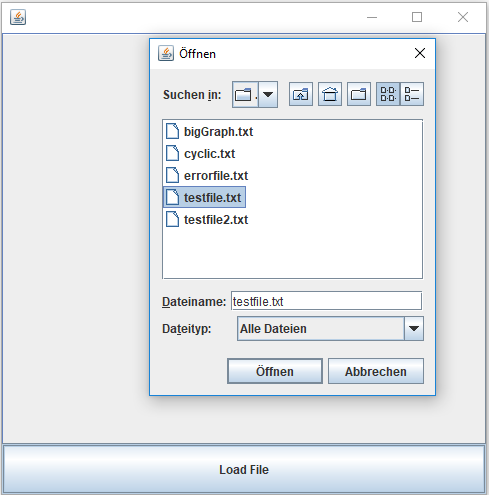
\includegraphics[width=.4\textwidth]{images/loadFile.png}
\end{figure}

Der \textit{Load File} Button ist auch noch dann sichtbar, wenn bereits Graphen geladen wurden. Öffnet man weitere Text Files, werden diese entsprechend in neuen Tabs geladen.

Ist das File kein Graph im Sinne unseres Eingabeformats oder ist der Graph nicht azyklisch, so wird eine Fehlermeldung ausgeben.

\subsection*{User Interface}

Hat der Benutzer einen gültigen Eingabegraphen ausgewählt und geöffnet, so stehen im mehrere Möglichkeiten zur Auswahl:

\begin{enumerate}
    \item[Anpassen der Fenstergrößen:] Alle Fenster können in ihrer Größe angepasst werden. Der Balken, der textuelle und graphische Ansicht der Graphen trennt, ist hierbei nur verschiebbar, wenn die Mindestgrößen der beiden Seiten nicht unterschritten werden.
   Das Panel, das die Steuerungselemente enthält kann per \textit{drag and drop} aus dem Fenster heraus- oder wieder hineingezogen werden.
    
    \item[Editieren des Graphen:] Auf der linken Seite des Fensters wird der Inhalt der geöffneten Textdatei angezeigt. Der Text kann modifiziert werden und die Änderungen durch das Klicken des \textit{Safe/Reload} Buttons gespeichert werden. Hierbei wird außerdem die Anzeige des Graphen neu geladen, so dass die vorgenommenen Änderungen sichtbar werden. 
    
    \textbf{Achtung! Erzeugt man hierbei einen ungültigen oder zyklischen Graphen, kann dies nur geändert werden, indem man außerhalb der Applikation die Datei öffnet und korrigiert!}
    
    \item[Graphen neu laden:] Den Knoten im Graphen werden zunächst Zufallskoordinaten zugewiesen, Dies kann dazu führen, dass sich Knoten beispielsweise überschneiden oder an einem Punkt häufen. Ist dergleichen der Fall, bietet es sich an den \textit{Safe/Reload} Button zu betätigen. Hierbei werden den Knoten neue Zufallskoordinaten zugewiesen.
    
    \item[Weitere Graphen öffnen:] Um weitere Graphen in neuen Tabs zu öffnen, kann der Benutzer den \textit{Load File} Button betätigen.
    
    \item[Justierungen vornehmen:] Die GUI stellt drei Slider bereit, die es dem Benutzer erlauben die Darstellung des Graphen und die Animation des Algorithmus anzupassen. Der \textit{Step Size} Slider legt fest, wie viele Berechnungsschritte auf ein mal ausgeführt werden sollen. Über Textfeld neben dem \textit{Step Size} Slider kann die Selbe Angabe gemacht werden. 
    
    Der \textit{Speed} Slider definiert wie schnell sich die Knoten in der Animation bewegen.
    
    Der \textit{Size} Slider setzt die Größe der Knoten fest und damit auch die Größe des Labels im Knoten.
    
    \item[Anzeige Speichern:] Per Rechtsklick auf die rechte Seite des Fensters (die den Graphen anzeigt) kann der Benutzer einen Snapshot der aktuellen Anzeige speichern.
    
    \item [Animation Starten/Stoppen:] Durch Drücken des \textit{play} Buttons kann der Benutzer die Animation starten, die entsprechend seiner Justierungen den Algorithmus auf den Graphen Ausführt. Durch Drücken auf den \textit{Pause} Button wird die Animation im aktuellen Schritt unterbrochen. 
    
    \item[Zurücksetzen:]Wird der \textit{Reset} Button gedrückt, so begeben sich die Knoten wieder zu ihren Ursprungspositionen und die Animation kann erneut gestartet oder der Algorithmus schrittweise verfolgt werden.
    
    \item[Schrittweises Ausführen:] Die Button \textit{Jump Forward} und \textit{Jump Backward} springen jeweils um so viele Berechnungsschritte vor oder zurück, wie über den \textit{Step Size} Slider angegeben wurde.
    
    
\end{enumerate}


\begin{figure}[ht!]
    \centering
    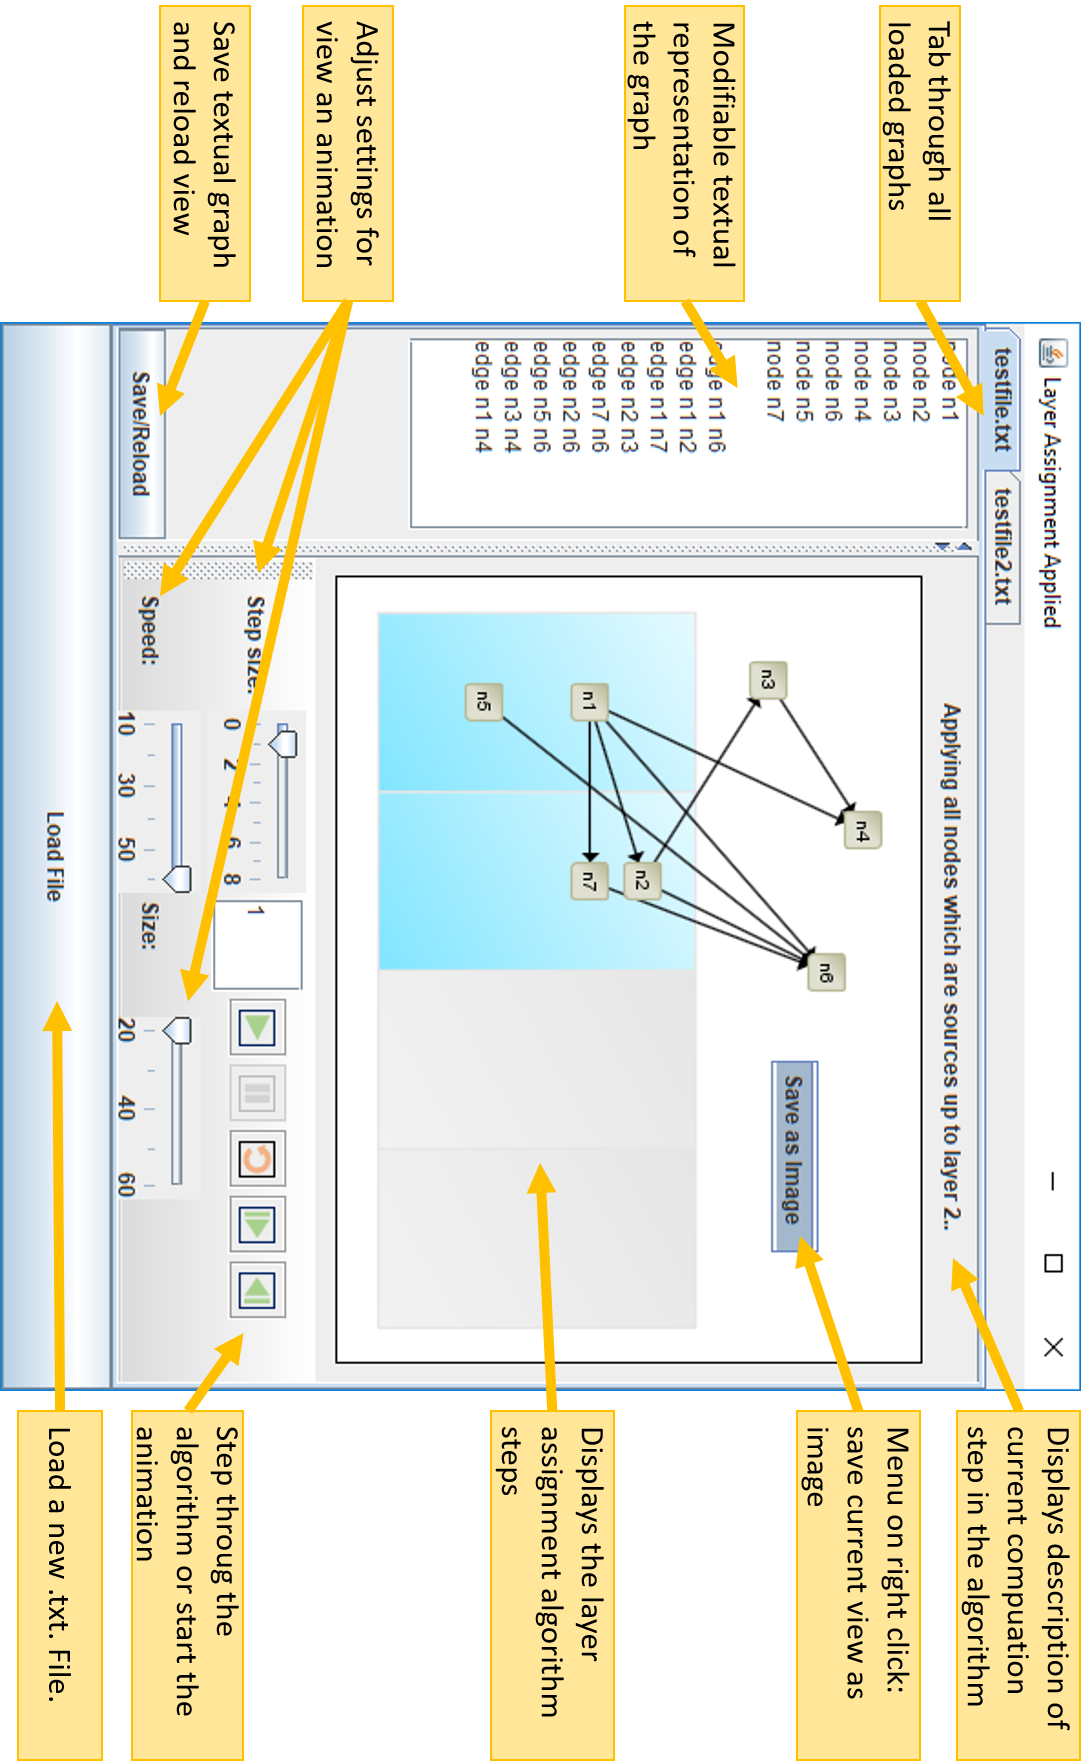
\includegraphics[width=\textwidth ]{images/toolGuide.png}
\end{figure}

    
    
    
    
    \section*{Visualisierung}
    


\subsection*{Visualize}











    
    
    
    
    
    
\end{document}






